\documentclass{beamer}

\usepackage[british]{babel}
\usepackage{graphicx,hyperref,ru,url}

% The title of the presentation:
%  - first a short version which is visible at the bottom of each slide;
%  - second the full title shown on the title slide;
\title[Linear-chain CRF for NLP in MADlib]{
  Linear-chain CRF for NLP in MADlib}

% The author(s) of the presentation:
%  - again first a short version to be displayed at the bottom;
%  - next the full list of authors, which may include contact information;
\author[Kun Li]{
  Kun Li \\\medskip
  {\small \url{kli@cise.ufl.edu}} \\ 
  {\small \url{http://www.cise.ufl.edu/~kli/}}}

% The institute:
%  - to start the name of the university as displayed on the top of each slide
%    this can be adjusted such that you can also create a Dutch version
%  - next the institute information as displayed on the title slide
\institute[University of Florida]{
  Department of Computer \& Information Science \& Engineering\\
  University of Florida}

% Add a date and possibly the name of the event to the slides
%  - again first a short version to be shown at the bottom of each slide
%  - second the full date and event name for the title slide
\date[Data Science Tea]{\today}

\begin{document}

\begin{frame}
  \titlepage
\end{frame}

\begin{frame}
  \frametitle{Outline}

  \tableofcontents
\end{frame}

% Section titles are shown in at the top of the slides with the current section 
% highlighted. Note that the number of sections determines the size of the top 
% bar, and hence the university name and logo. If you do not add any sections 
% they will not be visible.
\section{Introduction}

\begin{frame}
  \frametitle{Introduction}
  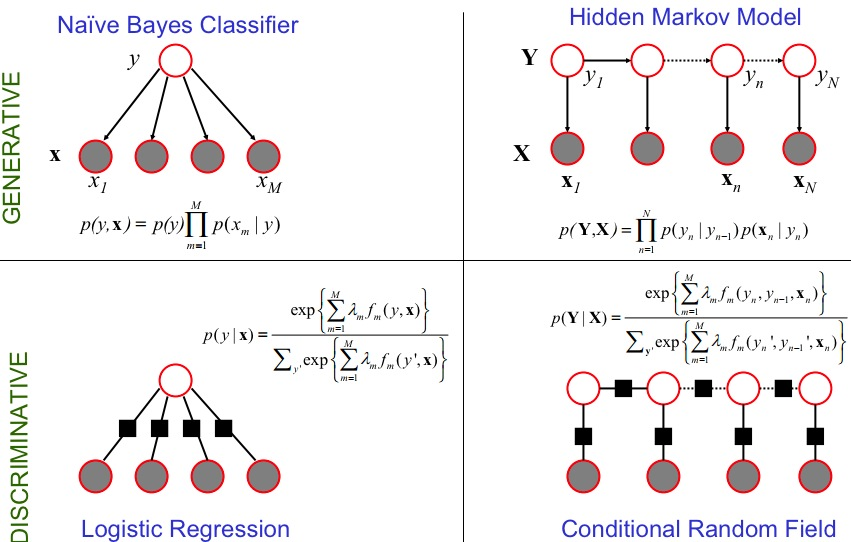
\includegraphics[height=11em]{models.jpg}\\
  \begin{itemize}
    \item Conditional probability p(label sequence y\|observation sequence x) rather than p(y,x)
    \item Allow arbitrary, non-independent features of the observation sequence X. 
  \end{itemize}
\end{frame}
\begin{frame}
  \frametitle{Introduction}
  \begin{center}
  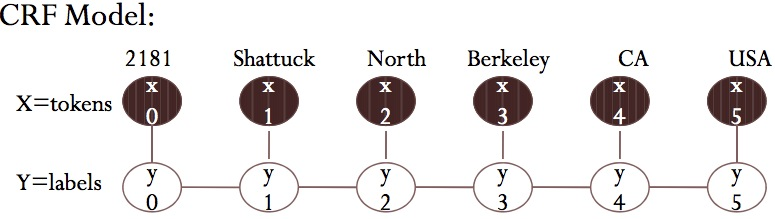
\includegraphics[height=10em, width=20em]{crf.jpg}\\
  \begin{tabular}{|l|c|c|}
  \multicolumn{3}{c}{\textbf{Table of strengths of DB and ML approaches}} \\
  \hline
  \textcolor{white}{X} & error & oov error \\
  \hline
  HMM & $5.69\%$ & $45.99\%$ \\
  \hline
  MEMM & $6.37\%$ & $54.61\%$ \\
  \hline
  CRF & $5.55\%$ & $48.05\%$ \\
  \hline
  \hline
  \end{tabular}
  \label{tab:approaches}
  \end{center}
\end{frame}

\section{System Achitecture}

\begin{frame}
  \frametitle{System Achitecture}
  \begin{center}
  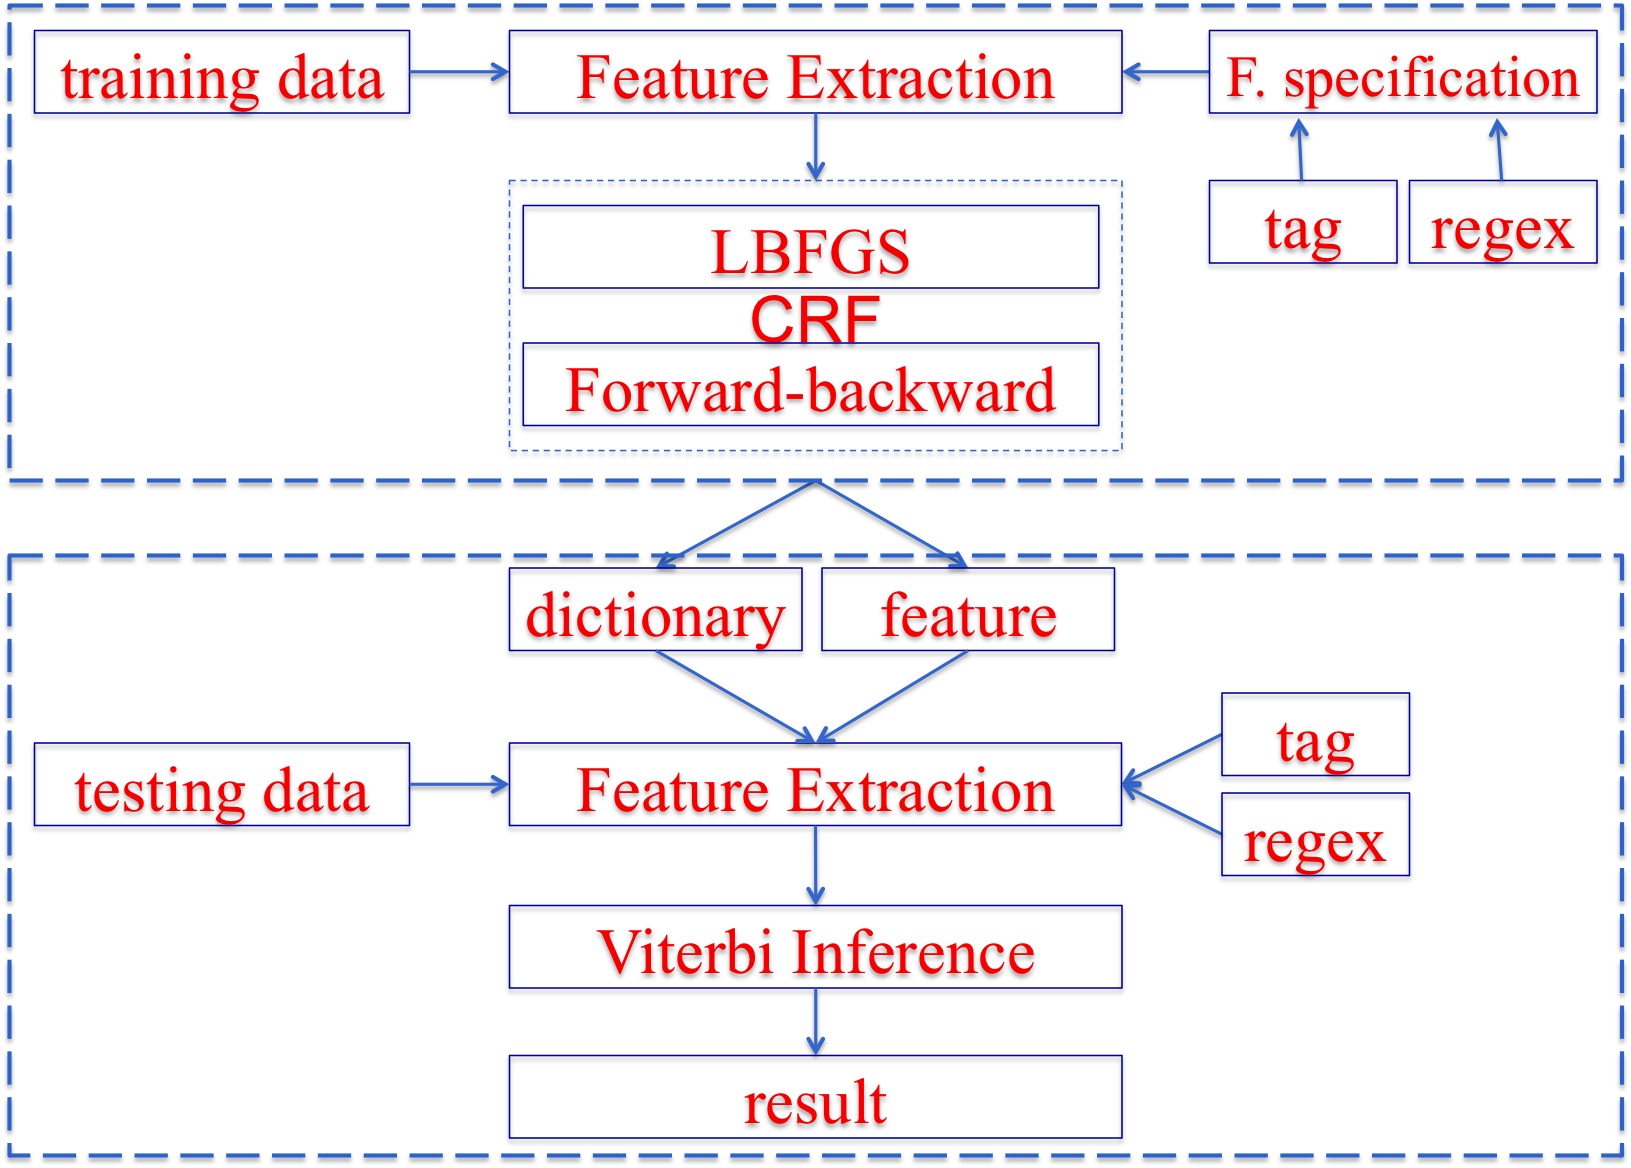
\includegraphics[height=18em]{system.png}
  \end{center}
\end{frame}


\section{Feature Extraction}
\begin{frame}
  \frametitle{Text Feature Extraction}
   \ Text feature extraction is a step in most statistical text analysis methods, and it can be an expensive operation. 
     To achieve high quality, CRF methods often assign tens of features to each token in the document. \\[1.5mm] 
     \textbf{\ Features}\vspace{-1.5mm}
     \begin{itemize}
      \item dictionary features: does this token exist in a provided dictionary? 
      \item regex features: does this token match a provided regular expression? 
      \item edge features: is the label of a token correlated with the label of a previous token? 
      \item word features: does this the token appear in the training data? 
      \item position features: is this token the first or last in the token sequence? 
     \end{itemize}
\end{frame}

\begin{frame}
  \frametitle{Training Feature Extraction}
  \begin{itemize}
  \item $INSERT INTO temp\_feature(start\_pos, doc\_id, fname,pre\_label,label)$\\ 
                        $SELECT start\_pos, doc\_id, 'R\_' || name, -1, label$\\
                        $FROM   textfex\_regex, textfex\_segmenttbl$\\
                        $WHERE  seg\_text ~ pattern$\\


  \item $INSERT INTO temp\_feature_index(fname,pre\_label,label)$\\ 
                        $SELECT DISTINCT ON fname, prev\_label\_id, label\_id$\\
                        $FROM   temp\_feature$\\


  \item $INSERT INTO feature(start\_pos, doc\_id, fname,pre\_label,label,f_index)$\\
                        $SELECT start\_pos, doc\_id, temp\_feature.fname, temp\_feature.prev\_label, temp\_feature.label, f\_index$\\
                        $FROM   temp\_feature, temp\_feature\_index$\\
  \end{itemize}
\end{frame}


\begin{frame}
  \frametitle{Testing Feature Extraction}
  \begin{itemize}
  \item Use $M$ table to encode edge features, position features. \\
  $M$ schema: $mtbl(prev\_label,label,value)$.
  \item Use $R$ table to encode single state features such as dictionary features, regex features.\\ 
  $R$ schema: $rtbl(seg\_text,label,value)$. \\
  \end{itemize}
  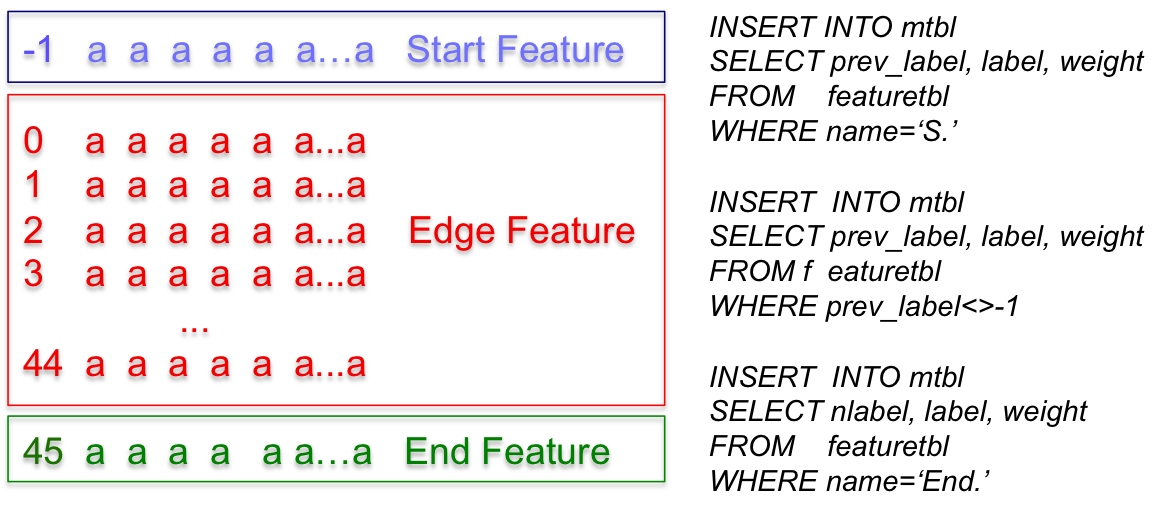
\includegraphics[height=7.02em]{m.png}\\
  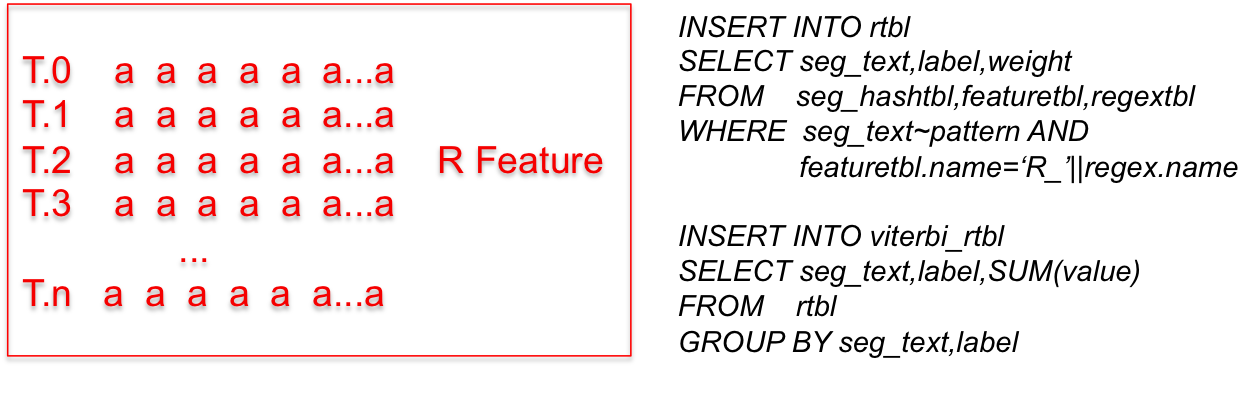
\includegraphics[height=5.85em]{r.png}\\
\end{frame}

\section{CRF training and Viterbi Inference}
\begin{frame}
  \frametitle{CRFs Objective Function}
  %\textbf{\ Features}\vspace{-1.5mm}
  $\max p_\theta (y|x) = \frac{\exp(\sum_j{\lambda_jt_j(y_{i-1},y_i,x,i) + \sum_k{\mu_k s_k(y_i,x,i))}}}
                        {\sum_y {\exp(\sum_j{\lambda_jt_j(y_{i-1},y_i,x,i) + \sum_k{\mu_k s_k(y_i,x,i))}}}}$\\
  \begin{itemize}
  \item $\theta=(\lambda_1,\lambda_2,...;\mu_1,\mu_2,...)$
  \item $t_j(y_{i-1},y_i,x,i)$ is a transition feature function of the entire observation sequence and the labels at positions $i$ and 
       $i-1$ in the label sequence
  \item $s_k(y_i,x,i)$ is a state feature function of the label at position $i$ and the observation sequence
  \item $\lambda_i$ and $\mu_k$ are parameters to be estimated from training data.
  \end{itemize}
\end{frame}

\begin{frame}
  \frametitle{Maximum Log\-likehood Principle}
  Train a CRF by maximizing the log-likelihood of a give training set $T={(x_k,y_k)}_{k=1}^N$\\
  $\max \ell_{\lambda}=\sum_k{(\lambda (F(y_k,x_k)-\log Z_\lambda(x_k))}$\\
  To perform this optimization, we seek the zero of the gradient\\
  $\nabla \ell_{\lambda}=\sum_k{(\lambda F(y_k,x_k)-E_{p\lambda(Y|x_k)}F(Y,x_k))}$\\
\end{frame}

\begin{frame}
  \frametitle{Parallel Training CRFs in MADlib}
  \fbox{%
        \parbox{0.95\linewidth}{%
1.Evaluate the log-likelihood function and gradient vector\\
$\ell_{\lambda_k}=\lambda F(y_k,x_k)-\log Z_\lambda(x_k)$(log-likelihood for doc. $k$)\\
$\nabla \ell_{\lambda_k}=\lambda F(y_k,x_k)-E_{p\lambda(Y|x_k)}F(Y,x_k)$(gradient vector for doc. $k$)\\
2.Sum up over all documents \\
$\ell_\lambda=\sum_k\ell_{\lambda_k}-\frac{\lambda^2}{2\sigma ^2}+const$(log-likelihood for all docs.)\\
$\nabla \ell_\lambda=\sum_k\nabla \ell_{\lambda_k}-\frac{\lambda}{\sigma ^2}$(gradient vector for all docs.)\\
3.Perform LBFGS optimization, a variation of quasi-Newton algorithm\\
$lbfgs(\lambda,\ell_\lambda,\nabla \ell_\lambda,Hessian,other args)$\\
4.Repeat step 1 and step2 until stop condition is satisfied
        }%
}\\
\end{frame}

\begin{frame}
  \frametitle{User Defined Aggregates}
  \begin{itemize}
\item madlib.crf\_gradient\_step\_transition(state,otherargs)RETURNS state


\item madlib.crf\_gradient\_step\_merge\_states(state ,state) RETURNS state


\item madlib.crf\_gradient\_step\_final(state) RETURNS state
  \end{itemize}
\end{frame}

\begin{frame}
  \frametitle{Forward-backward algorithm}
  The expectation $E_{p\lambda(Y|x_k)}F(Y,x)$ can be computed efficiently using a variant of the forward-backward algorithm.
For a given x, define the transition matrix for position i as \\
$M_i[y,y^\prime]=\exp \lambda f(y,y^\prime,x,i)$\\
$Let f be any local feature, f_i[y,y^\prime]=f(y,y^\prime,x,i),$
$F(y,x)=\sum_i{f(y_{i-1},y_i,x,i)}, and let * denote component-wise matrix product, then$\\
$E_{p\lambda(Y|x_k)}F(Y,x)=\sum_y{p_\lambda(y|x)F(y,x)}$\\
$=\sum_i{\frac{a_{i-1}(f_i*M_i)\beta_i^T}{Z_\lambda(x)}}$\\
\begin{itemize}
\item $Z_\lambda(x)=a_n \cdot 1^T$
\item $a_i=$
\item $\beta_i^T=$
\end{itemize}
Use a forward pass to compute the $a_i$ and a backward pass to compute $\beta_i$ and accumulate the feature expectations.
\end{frame}

\begin{frame}
  \frametitle{The limited-memory BFGS}
  $f_T(x_n+\nabla x)=f_T(x)=f(x_n)+f^\prime(x_n)\nbla x +1/2f\prime\prime(x_n)\nblax^2$\\
  $f^\prime(x_n)+f^\prime\prime(x_n)\nblax x=0;$
  $x_{n+1} = x_n - \frac{f^\prime(x_n)}{f^\prime\prime(x_n)},n=0,1,..$\\
  will converge towards a root of $f_prime(x)=0$
  \begin{center}
  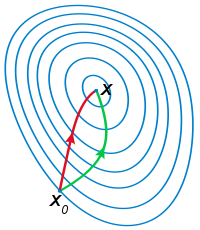
\includegraphics[height=8em]{newton_grad.png}
  \end{center}
 LBFGS\\
 
\end{frame}

%\section{Viterbi Inference}
\begin{frame}
  \frametitle{Viterbi Inference}
  The Viterbi algorithm is the popular algorithm to find the top-k most likely labelings of a document 
for CRF models. 
We chose to implement a Python UDF that uses iterations to drive the Viterbi inference. Each iteration will 
finish the inference over one document.
In Greenplum, Viterbi can be run in parallel over different subsets 
of the document on a multi-core machine.
\[
V(i,y) =
\begin{cases}
 \max_{y^\prime}(V(i-1,y^\prime)) + \textstyle \sum_{k=1}^K \lambda_kf_k(y,y^\prime,x_i), & \text{if } i\ge0 \\
 0, & \text{if } i=-1.
\end{cases}
\]
\begin{center}		             
  %\begin{multicols}{2}
      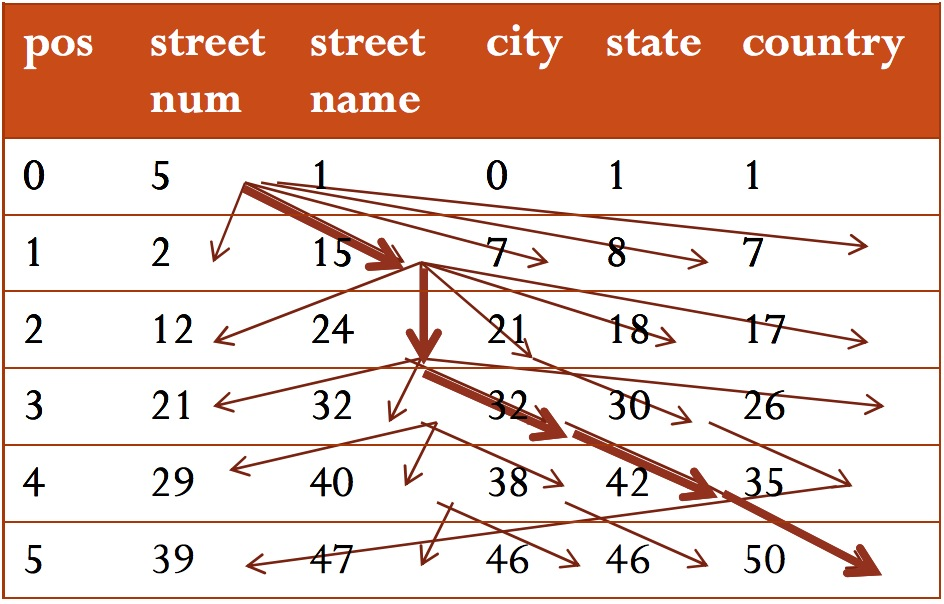
\includegraphics[height=5em,width=11em]{viterbip.jpg}
      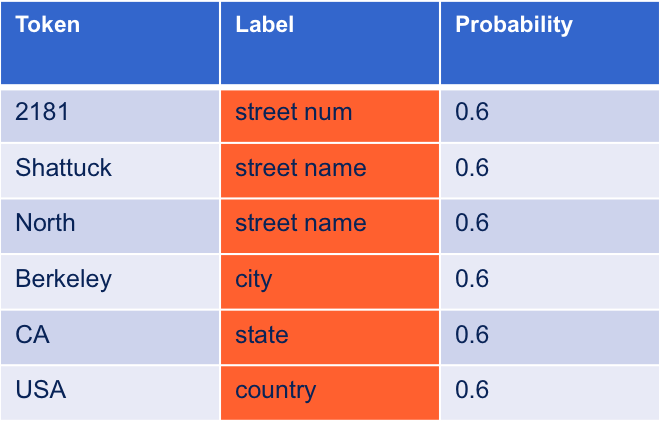
\includegraphics[height=5em,width=11em]{result.png}\\
  %\end{multicols}
\end{center}
\end{frame}

\section{Conclusion and Future Work}

\begin{frame}
  \frametitle{Conclusion and Future Work}

  \begin{itemize}
    \item SELECT madlib.traindata\_textfex(args)
    \item SELECT madlib.testdata\_textfex(args)
    \item SELECT madlib.linear\_crf\_training(args)
    \item SELECT madlib.viterbi\_inference(args)
  \end{itemize}
  System: \textcolor{green}{Postgres} VS \textcolor{blue}{Greenplum(2 segments)}\\
	  Text Feature Extraction + Viterbi Inference
	  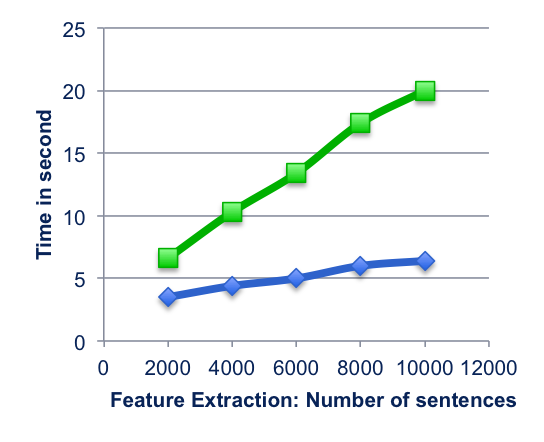
\includegraphics[height=9.9em]{extraction.png}
	  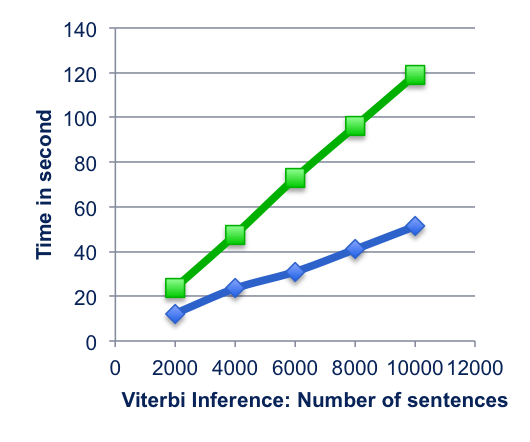
\includegraphics[height=9.9em]{viterbi.png}
\end{frame}

\begin{frame}
  \frametitle{Questions}
  \begin{center}
   Thanks! Questions?
  \end{center}
\end{frame}

\end{document}
